\begin{frame}[plain]
  \vfill
  \centering
  \Huge Multimodal Architectures
  \vfill
\end{frame}

\begin{frame}{Categories of Multimodal Architectures}
  \begin{itemize}
    \item[\textcolor{red}{$\triangleright$}] \textbf{Early Fusion:} Combine the modalities at the input of a
      single shared model.\\
      \textit{Then: VisualBERT added detector regions as input tokens. Now: Chameleon and Llama 4
      pretrain on mixed token sequences from the start.}
    \item[\textcolor{red}{$\triangleright$}] \textbf{Late Fusion (dual encoder):} Process each modality
      separately, then merge only at the output.\\
      \textit{CLIP and SigLIP: right for retrieval and zero-shot scoring, too weak for generation.}
    \item[\textcolor{red}{$\triangleright$}] \textbf{Middle Fusion / Cross-modal Attention:} Let the modalities
      interact inside the stack.\\
      \textit{Flamingo's gated cross-attention; the projector recipe merges at the token level instead,
      early fusion around an unchanged LLM.}
  \end{itemize}

  \vspace{0.6em}
  \textbf{Design Considerations:}
  \begin{itemize}
    \item[\textcolor{red}{$\triangleright$}] \textbf{Alignment:} How to align representations across modalities.
    \item[\textcolor{red}{$\triangleright$}] \textbf{Modality Dropout:} Handling missing or noisy modalities during training or inference.
    \item[\textcolor{red}{$\triangleright$}] \textbf{Shared vs. Modality-Specific Layers:} Deciding which layers are shared and which are unique to each modality.
  \end{itemize}
\end{frame}

\begin{frame}{Where Fusion Happens}
  \begin{figure}
    \centering
    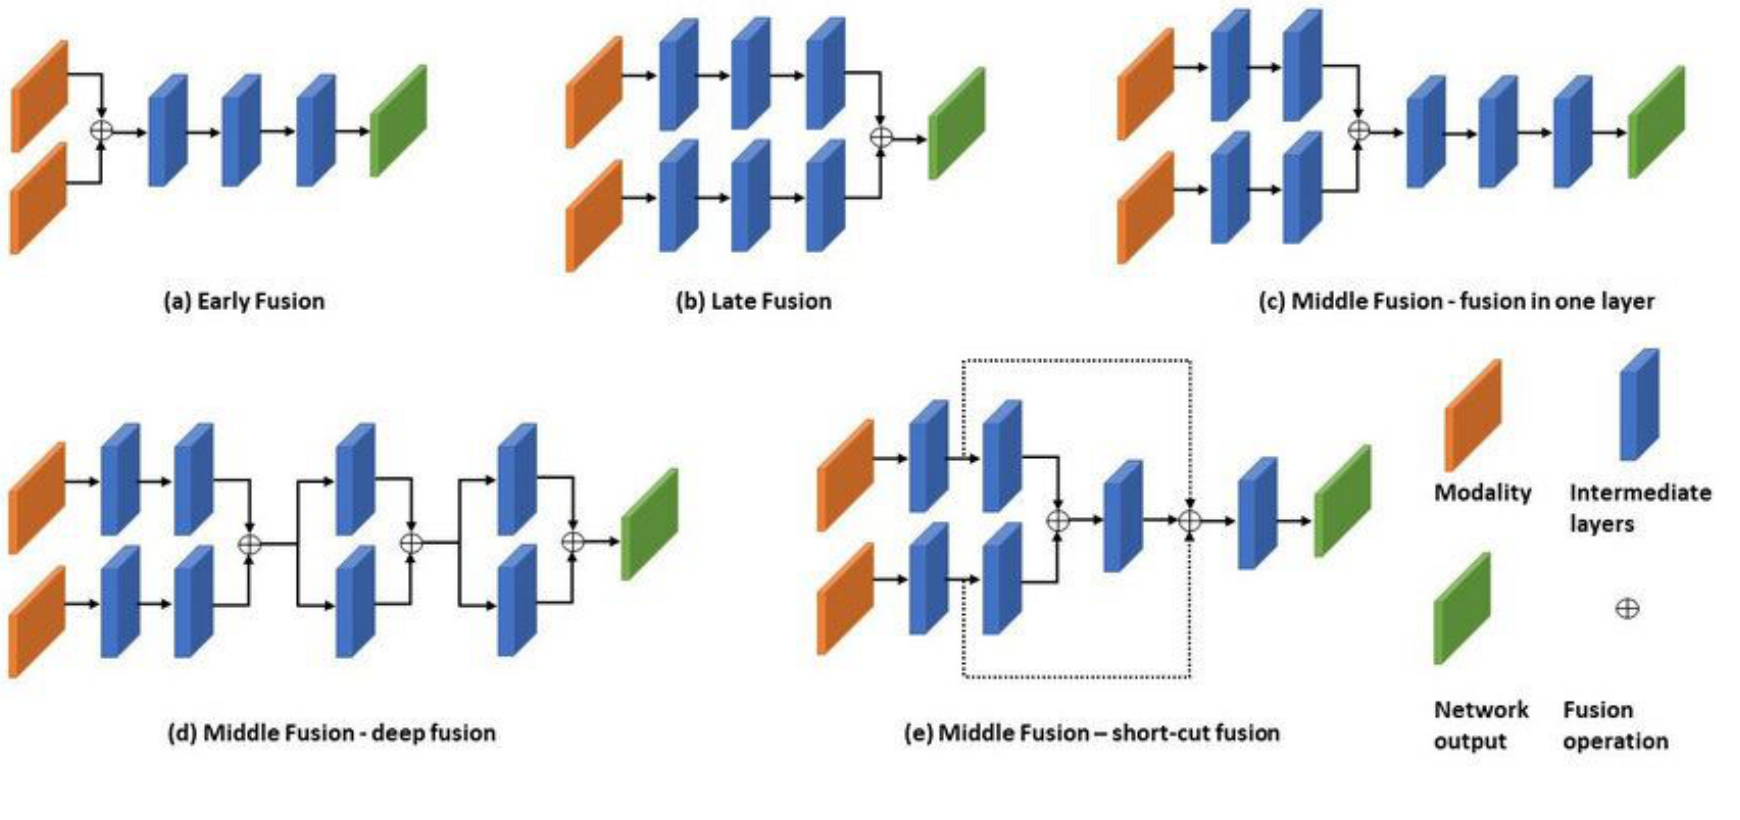
\includegraphics[width=0.98\textwidth, height=0.78\textheight, keepaspectratio]{images/multimodal-nlp/multimodal_fusion_strategies_diagram.png}
    \caption*{\scriptsize Orange is a modality, blue an intermediate layer, green the network output, and
    $\oplus$ a fusion operation. Middle fusion is the general case: the hybrid, cross-modal-attention
    designs sit here. Source: Feng et al., ``Deep Multi-modal Object Detection and Semantic Segmentation
    for Autonomous Driving'', \href{https://arxiv.org/abs/1902.07830}{arXiv:1902.07830}, Figure~8.}
  \end{figure}
\end{frame}

\begin{frame}{Challenges in Multimodal Integration}
  \begin{figure}
    \centering
    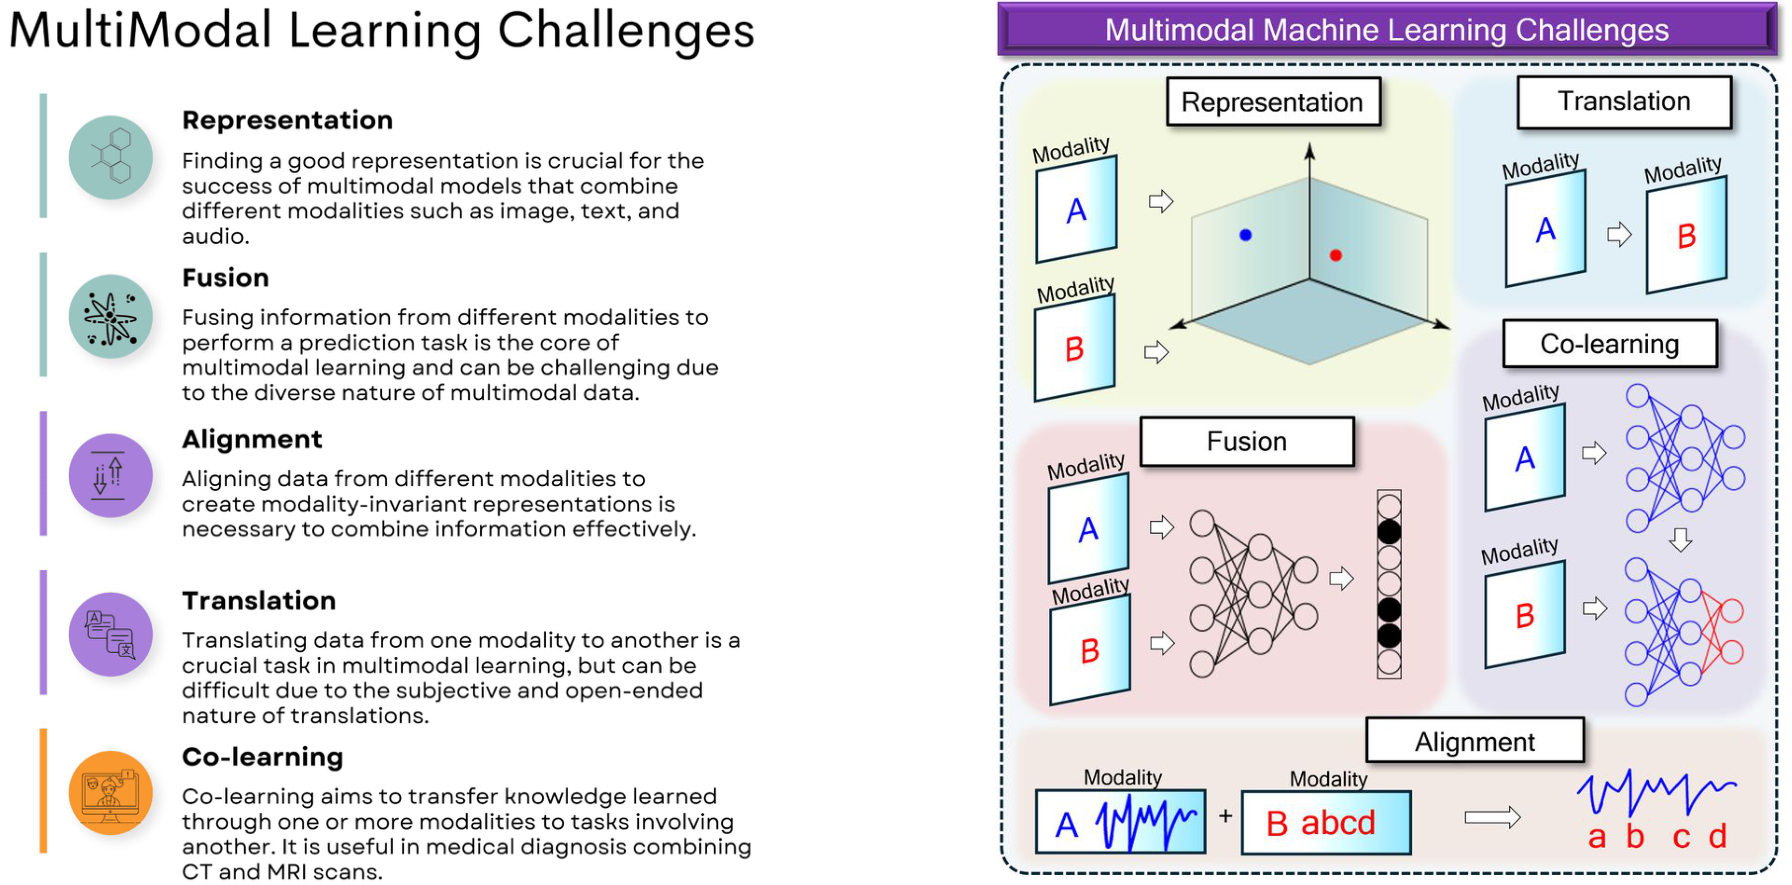
\includegraphics[width=0.98\textwidth, height=0.78\textheight, keepaspectratio]{images/multimodal-nlp/multimodal_learning_challenges.png}
    \caption*{\scriptsize Representation, fusion, alignment, translation and co-learning: the five-way
    taxonomy of Baltru\v{s}aitis, Ahuja \& Morency, ``Multimodal Machine Learning: A Survey and Taxonomy'',
    \href{https://arxiv.org/abs/1705.09406}{arXiv:1705.09406}. Object hallucination is an alignment
    failure; omni models are translation at work; the taxonomy predates them all and still fits.}
  \end{figure}
\end{frame}
